\chapter{Implementation} % The implementation should look at any issues you encountered as you tried to implement your design. During the work, you might have found that elements of your design were unnecessary or overly complex; perhaps third party libraries were available that simplified some of the functions that you intended to implement. If things were easier in some areas, then how did you adapt your project to take account of your findings? It is more likely that things were more complex than you first thought. In particular, were there any problems or difficulties that you found during implementation that you had to address? Did such problems simply delay you or were they more significant? You can conclude this section by reviewing the end of the implementation stage against the planned requirements.

@TODO - style guide


\section{SmartResolution directory structure}

As the implementation followed an agile methodology, the design evolved over time and thus, the directory structure could not be determined up-front. Most (but not all) of the key directories and folders are outlined below:

\begin{samepage}
\dirtree{%
.1 data/.
.1 features/.
.1 test/.
.1 vendor/.
.1 webapp/.
.2 core/.
.3 api/.
.3 controller/.
.3 db/.
.3 model/.
.3 view/.
.2 modules/.
.3 other/.
.3 config.json.
.2 uploads/.
.2 index.php.
.2 routes.php.
.1 .travis.yml.
.1 composer.json.
.1 Gemfile.
}
\end{samepage}

\lstinline{data} contains fixture data for tests. This is also where the test and production SQLite3 databases reside.

\lstinline{features} contains the Cucumber features and Ruby step definitions.

\lstinline{test} contains all PHP unit tests.

\lstinline{vendor} is an automatically generated directory, created by Composer, containing all of SmartResolution's dependencies.

\lstinline{webapp/core} contains the core ODR platform, which uses an MVCR compound design pattern (\lstinline{webapp/routes.php} defines the routing component). The \lstinline{model}, \lstinline{view} and \lstinline{controller} directories are self-explanatory.

Also inside the core is the \lstinline{db} directory, which contains middleware classes connecting the model classes to the database, since models should encapsulate the concept of whatever it is they are representing, rather than being responsible for the relational database to object mapping.

Finally, this folder also contains an \lstinline{api} directory, which defines all of the global functions available to modules. Having these in their own directory made generating module-specific API documentation easy.

Going back up a level, we have \lstinline{webapp/modules}, which contains any installed SmartResolution modules. This is where the maritime collision module resides once it has been installed. A \lstinline{config.json} file (edited in a user-friendly way through the admin dashboard) denotes which modules are installed and whether or not they are active.

Finally, at the top level we have a few interesting files:

\lstinline{.travis.yml} - an instructions file for Travis Continuous Integration, describing how to set up the project and run its tests.

\lstinline{composer.json} - describes SmartResolution's dependencies. Developers can install all dependencies simply by running \lstinline{composer install}.

\lstinline{Gemfile} - describes SmartResolution's Ruby dependencies. Required for the Cucumber and Ruby integration tests.

\section{Class diagrams}

The system was developed in an agile way, hence these class diagrams are not in the design section but the implementation section. What evolved from the design was a state pattern representing the current state of a dispute.

Please refer to figures~\ref{uml:activity:dispute} and~\ref{uml:activity:mediation} for a reminder of the workflow of a dispute. These diagrams alluded to the fact that disputes can be in different states. This was something that carried over to the implementation of the code.

\begin{figure}[h!]
  \centering
    \ifimages
    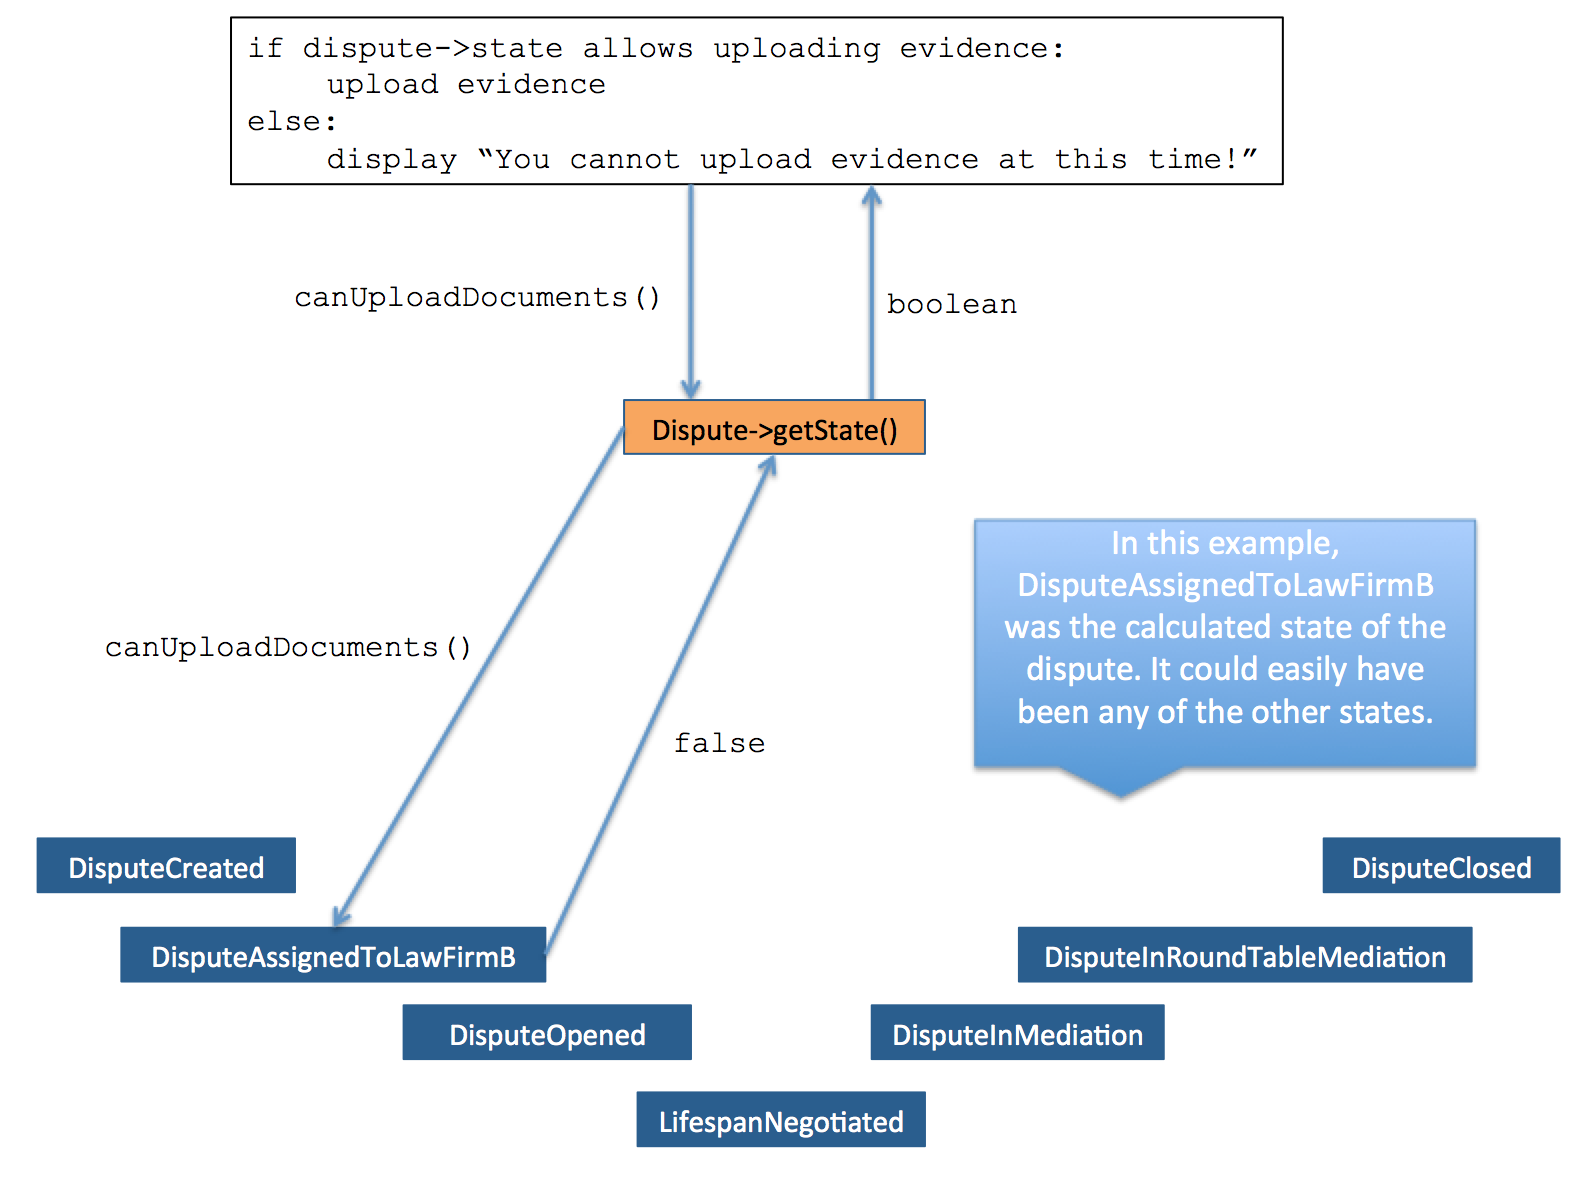
\includegraphics[width=\textwidth]{states}
    \fi
  \caption{Visualisation of how the state pattern works in SmartResolution}
  \label{uml:states}
\end{figure}

Figure~\ref{uml:states} shows how the classes throughout SmartResolution can query a dispute's state to ask permission regarding certain actions, rather than hard-coding something like:

\begin{lstlisting}
if ($dispute->state() === 'Open' || $dispute->state() === 'InMediation' || // etc) {
    // some action
}
\end{lstlisting}

The list of possible states are as follows:

\begin{itemize}
    \item \textbf{DisputeCreated} - this is the very first state of the dispute, having just been created.
    \item \textbf{DisputeAssignedToLawFirmB} - this rather long-winded name represents the state of the dispute when it has just been assigned to the other law firm. At this stage, one dispute party is complete, whilst the other only has the law firm. We are still waiting for the law firm to assign an agent.
    \item \textbf{DisputeOpened} - all law firms and agents have been assigned. Now a lifespan must be negotiated.
    \item \textbf{LifespanNegotiated} - the agents have managed to negotiate a lifespan and there is nothing more to do to initiate the dispute. When the start date is surpassed, the dispute is underway and the agents are free to perform all dispute-related actions. When the end date passes, the dispute is automatically closed.
    \item \textbf{DisputeInMediation} - the agents have decided to put the dispute into mediation and have negotiated a mediation centre and a mediator. It is important to note that not all disputes will necessarily reach this stage.
    \item \textbf{DisputeInRoundTableMediation} - all parties are free to communicate openly. By default, a dispute in mediation disables direct communication between the two agents. The mediator can enable round-table communication to put the dispute into this state.
    \item \textbf{DisputeClosed} - the dispute is now closed, either because an agent closed it or because the lifespan of the dispute came to an end.
\end{itemize}


Also

@TODO - a class diagram showing all classes

Also

@TODO - describe in detail the models, data mappers and controller objects.

\section{Routing}

@TODO - before this point, describe the classes etc, since these are alluded to in the diagram.

\begin{figure}[h!]
  \centering
    \ifimages
    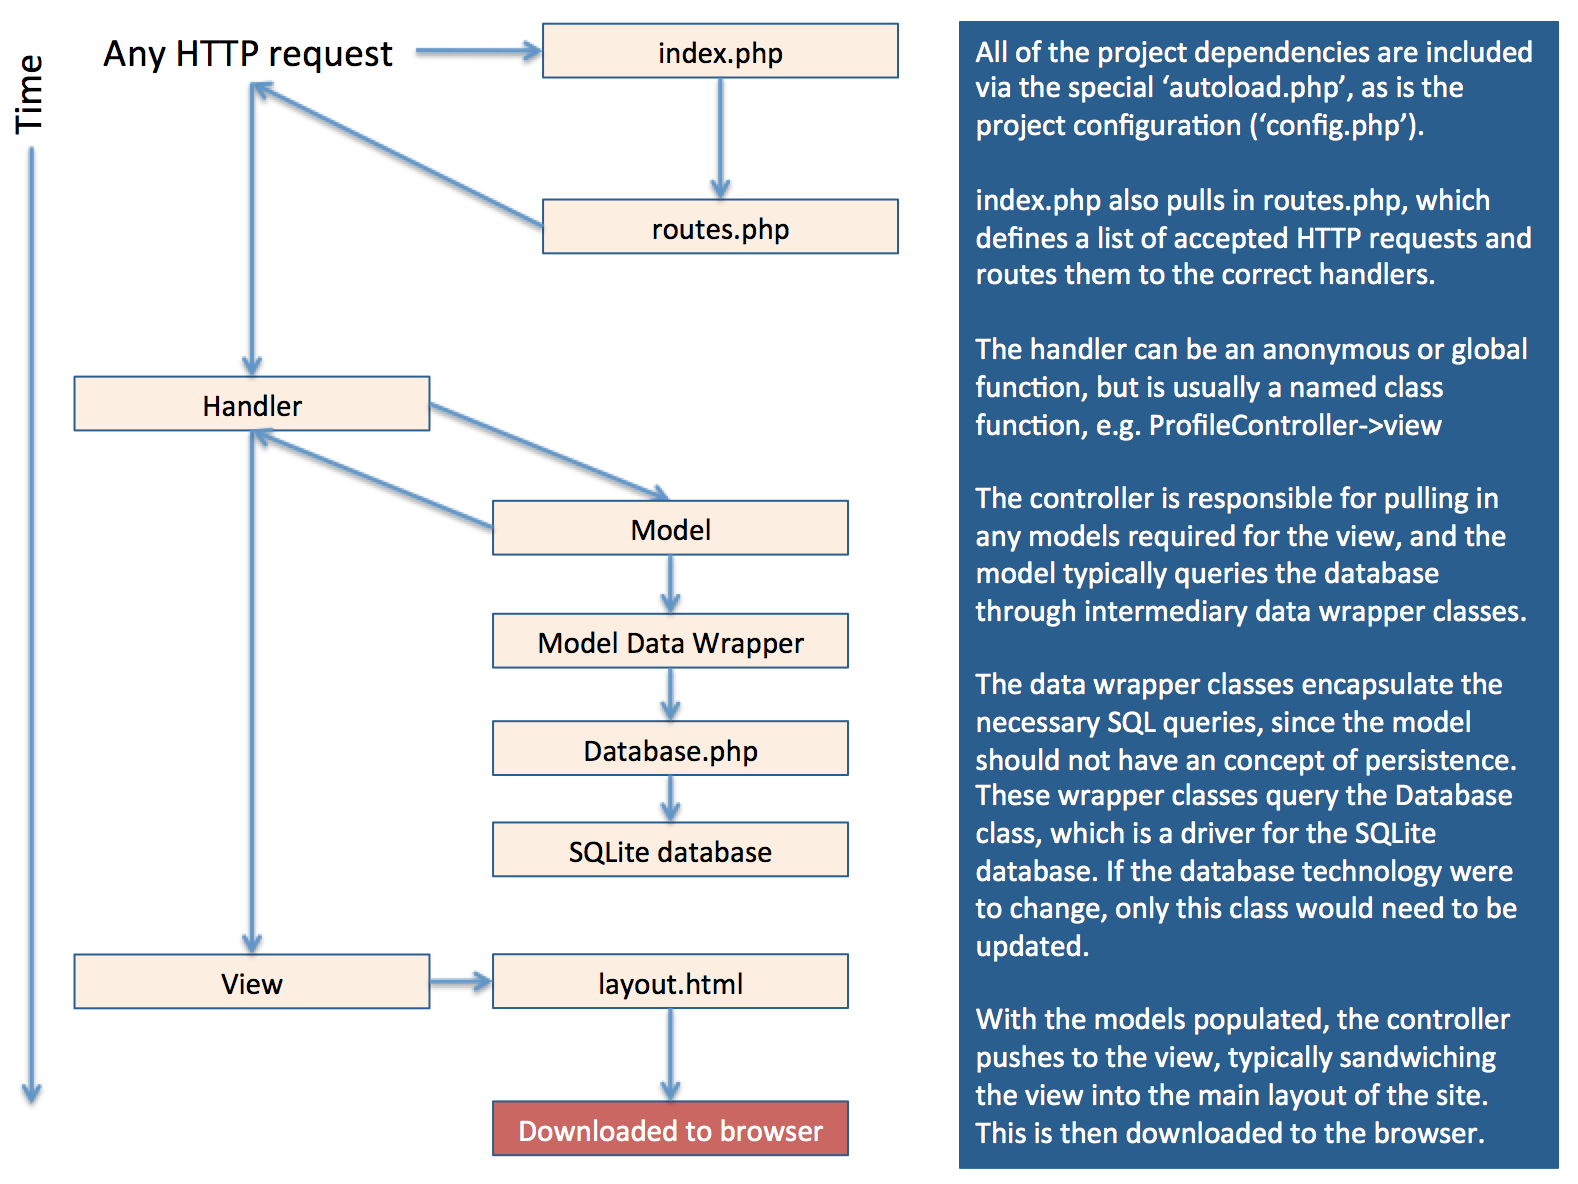
\includegraphics[width=\textwidth]{routing}
    \fi
  \caption{How SmartResolution processes HTTP requests}
  \label{uml:routing}
\end{figure}

Figure~\ref{uml:routing} shows how SmartResolution routes HTTP requests and renders data-driven pages. As described in the image, the HTTP request is processed by \lstinline{routes.php} and forwarded to the appropriate controller, which then instantiates the models and renders the view.

\section{Comments}

@TODO mention this somewhere:

The codebase is liberally commented throughout, using API-style markup. This was a difficult decision, discussed and justified in appendix~\ref{appendix:comments}.